%===================================
% KEY SUMMARY — Tutorial 10 Concepts
%===================================



\section*{Simulink Problem-Solving and Manual Drawing Framework(Tutorial 10)}

\vspace{0.5cm}

%================================================================
% 1. DIRECT INTEGRATION
%================================================================
\section*{1. The Direct Integration Framework (For Standard ODEs)}
\textbf{Applies to:} Problems 3, 5, 8, 33

This framework is used when you are dealing with standard, time-domain differential equations containing $\dot{y}$ or $\ddot{y}$.

\subsection*{Problem-Solving Steps}
\begin{enumerate}
    \item \textbf{Isolate the highest derivative:} Algebraically rearrange the equation so the highest derivative is alone on the left side of the equals sign. For example, in Problem 8, $10\ddot{y} = 7\sin(4t) + 5\cos(3t)$ would become $\ddot{y} = \frac{1}{10}(7\sin(4t) + 5\cos(3t))$.
    \item \textbf{Chain your Integrators:} For a second-order equation ($\ddot{y}$), place two Integrator ($\frac{1}{s}$) blocks in series.
    \item \textbf{Build the feedback loops:} Tap the output signals ($y$ or $\dot{y}$) and route them backward through Gain blocks (triangles) to construct the rest of the equation.
    \item \textbf{Sum it up:} Feed the inputs and the feedback loops into a Sum block ($+$/$-$), and connect the Sum block's output directly into your first Integrator.
\end{enumerate}

\subsection*{Manual Drawing Guidelines}
\textbf{Shapes to Draw:}
\begin{itemize}
    \item \textbf{Integrators:} Draw a square and write $\frac{1}{s}$ inside it.
    \item \textbf{Gains (Multipliers):} Draw a triangle pointing to the right. Write the constant multiplier (e.g., $5$ or $\frac{1}{3}$) inside it.
    \item \textbf{Sum Junctions:} Draw a circle. Write small $+$ and $-$ signs inside the circle next to where the arrows will enter to show addition or subtraction.
    \item \textbf{Math Functions:} Draw a square and write the function name inside (e.g., $\sin$, $\cos$, $\tan$).
\end{itemize}

\textbf{How to Draw the Process (Example: $3\dot{y} + 5\sin y = f(t)$):}
\begin{itemize}
    \item \textbf{Isolate:} Mentally rearrange to $\dot{y} = \frac{1}{3}(f(t) - 5\sin y)$.
    \item \textbf{The Spine:} Draw an Integrator ($\frac{1}{s}$) in the middle of the page. Draw an arrow exiting the right side and label the line $y(t)$.
    \item \textbf{The Feedback:} Tap the $y(t)$ line, draw an arrow looping back to the left, and pass it through a square labeled $\sin$, then through a triangle labeled $5$.
    \item \textbf{The Summation:} Draw a circle (Sum junction) to the left of the Integrator. Draw an arrow from your input $f(t)$ into a $+$ port. Bring the arrow from your $5$ triangle into a $-$ port.
    \item \textbf{The Final Gain:} Draw an arrow from the Sum circle through a triangle labeled $\frac{1}{3}$, and plug that arrow into the Integrator.
\end{itemize}

\begin{figure}[H]
    \centering
    \begin{tikzpicture}[>=Stealth]
        
        % Define standard block styles
        \tikzset{
            block/.style = {draw, rectangle, minimum height=1cm, minimum width=1.2cm, align=center, fill=blue!5},
            sum/.style = {draw, circle, minimum size=0.8cm, inner sep=0pt, fill=blue!5},
            gain/.style = {draw, regular polygon, regular polygon sides=3, shape border rotate=-90, minimum width=1cm, inner sep=0pt, fill=blue!5},
            gainleft/.style = {draw, regular polygon, regular polygon sides=3, shape border rotate=90, minimum width=1cm, inner sep=0pt, fill=blue!5},
            panel/.style = {draw, rectangle, rounded corners, minimum width=14.5cm, fill=gray!5, dashed} 
        }

        %=========================================
        % STEP 1: ISOLATE
        %=========================================
        % Centered at y=0, height 2.5cm
        \node [panel, minimum height=2.5cm] (p1) at (0,0) {};
        \node [anchor=north west, font=\bfseries] at (p1.north west) {Step 1: Isolate the highest derivative};
        
        \node [anchor=center, font=\Large] at (p1.center) {
            $m\ddot{y} + c\dot{y} + ky = f(t) \quad \Rightarrow \quad \ddot{y} = \frac{1}{m} \big[ f(t) - c\dot{y} - ky \big]$
        };

        %=========================================
        % STEP 2: CHAIN INTEGRATORS
        %=========================================
        % Centered at y=-4, height 2.5cm
        \node [panel, minimum height=2.5cm] (p2) at (0,-4) {};
        \node [anchor=north west, font=\bfseries] at (p2.north west) {Step 2: Chain your Integrators};
        
        \node [block] (int1_s2) at (-1.5, -4.2) {$\frac{1}{s}$};
        \node [block] (int2_s2) at (1.5, -4.2) {$\frac{1}{s}$};
        
        \draw [->, thick] (-3.5, -4.2) -- node[above] {$\ddot{y}$} (int1_s2);
        \draw [->, thick] (int1_s2) -- node[above] {$\dot{y}$} (int2_s2);
        \draw [->, thick] (int2_s2) -- node[above] {$y$} (3.5, -4.2);

        %=========================================
        % STEP 3: BUILD FEEDBACK
        %=========================================
        % Centered at y=-9.25, height 4.5cm to accommodate the loop
        \node [panel, minimum height=4.5cm] (p3) at (0, -9.25) {};
        \node [anchor=north west, font=\bfseries] at (p3.north west) {Step 3: Build the feedback loops (Tap and Gain)};
        
        \node [block] (int1_s3) at (-1.5, -8.5) {$\frac{1}{s}$};
        \node [block] (int2_s3) at (1.5, -8.5) {$\frac{1}{s}$};
        \node [gainleft] (gainC) at (-0.5, -10.2) {$c$};
        \node [gainleft] (gainK) at (1, -10.2) {$k$};
        
        \draw [->, thick] (-3.5, -8.5) -- node[above] {$\ddot{y}$} (int1_s3);
        \draw [->, thick] (int1_s3) -- node[above] {$\dot{y}$} (int2_s3);
        \draw [->, thick] (int2_s3) -- node[above] {$y$} (3.5, -8.5);
        
        % Taps
        \filldraw (0, -8.5) circle (2pt);
        \draw [->, thick] (0, -8.5) |- (gainC.east);
        
        \filldraw (2.8, -8.5) circle (2pt);
        \draw [->, thick] (2.8, -8.5) |- (gainK.east);

        %=========================================
        % STEP 4: SUM IT UP
        %=========================================
        % Centered at y=-15.5, height 6cm to accommodate double loops and Sum junction
        \node [panel, minimum height=6cm] (p4) at (0, -15.5) {};
        \node [anchor=north west, font=\bfseries] at (p4.north west) {Step 4: Sum it up (Combine and plug into the front)};
        
        \node [sum] (sum_s4) at (-4.5, -14) {};
        \node [font=\tiny] at ($(sum_s4.west)+(0.15,0.1)$) {$+$};
        \node [font=\tiny] at ($(sum_s4.south)+(0.1,0.15)$) {$-$};
        \node [font=\tiny] at ($(sum_s4.south east)+(-0.05,0.25)$) {$-$};
        
        \node [gain] (gainM) at (-2.5, -14) {1/m};
        \node [block] (int1_s4) at (0, -14) {$\frac{1}{s}$};
        \node [block] (int2_s4) at (3, -14) {$\frac{1}{s}$};
        
        \node [gainleft] (gainC4) at (0, -15.8) {$c$};
        \node [gainleft] (gainK4) at (1.5, -17.2) {$k$};
        
        % Forward Path
        \draw [->, thick] (-6.5, -14) node[left] {$f(t)$} -- (sum_s4);
        \draw [->, thick] (sum_s4) -- (gainM);
        \draw [->, thick] (gainM) -- node[above] {$\ddot{y}$} (int1_s4);
        \draw [->, thick] (int1_s4) -- node[above] {$\dot{y}$} (int2_s4);
        \draw [->, thick] (int2_s4) -- node[above] {$y$} (5, -14);
        
        % Feedback Paths
        \filldraw (1.5, -14) circle (2pt);
        \draw [->, thick] (1.5, -14) |- (gainC4.east);
        \draw [->, thick] (gainC4.west) -| (sum_s4.south);
        
        \filldraw (4.2, -14) circle (2pt);
        \draw [->, thick] (4.2, -14) |- (gainK4.east);
        \draw [->, thick] (gainK4.west) -| ($(sum_s4.south east)+(-0.15,-0.15)$);

    \end{tikzpicture}
    \caption{The 4-Step Direct Integration Framework}
\end{figure}


\vspace{0.5cm}

%================================================================
% 2. TRANSFER FUNCTIONS
%================================================================
\section*{2. The Transfer Function Framework (For LTI Systems)}
\textbf{Applies to:} Problems 25, 28

This framework is used for Linear Time-Invariant (LTI) systems, specifically when initial conditions are zero.

\subsection*{Problem-Solving Steps}
\begin{enumerate}
    \item \textbf{Convert to Laplace:} Take the Laplace transform of the differential equations, assuming zero initial conditions.
    \item \textbf{Define Polynomials:} Structure the equation into a ratio of polynomials ($\frac{\text{Numerator}}{\text{Denominator}}$) to find the transfer function, such as $\frac{X(s)}{F(s)} = \frac{1}{3s^2+15s+18}$.
    \item \textbf{Block Setup:} Use the Transfer Fcn block. You must input the coefficients of the $s$-polynomials into the block parameters in descending order.
    \item \textbf{Connect Input/Output:} Connect your input source (e.g., a Step block) to the front. If you have a cascaded system like Problem 25, you chain the Transfer Function blocks together.
\end{enumerate}

\subsection*{Manual Drawing Guidelines}
\textbf{Shapes to Draw:}
\begin{itemize}
    \item \textbf{Transfer Function:} Draw a wide rectangle. Inside, draw a horizontal line and write the numerator on top and the denominator on the bottom (e.g., $\frac{1}{3s^2+15s+18}$).
    \item \textbf{Multiplexer (Mux):} If you need to output two signals to the same scope, draw a thick, solid black vertical line.
    \item \textbf{Inputs/Outputs:} Draw squares labeled ``Step'' or ``Ramp'' for inputs, and ``Scope'' or ``simout'' for outputs.
\end{itemize}

\textbf{How to Draw the Process:}
\begin{itemize}
    \item Draw the input block on the far left (e.g., a ``Step'' block).
    \item Draw your wide Transfer Function rectangle(s) in the middle.
    \item Draw standard straight arrows connecting them from left to right.
\end{itemize}

\vspace{0.5cm}
% 
%================================================================
% 3. STATE-SPACE
%================================================================
\section*{3. The State-Space Framework (For Coupled First-Order ODEs)}
\textbf{Applies to:} Problems 13, 15, 45a

This approach is required when the system is given as a system of coupled first-order differential equations, or when specifically asked to use state-variable representation.

\subsection*{Problem-Solving Steps}
\begin{enumerate}
    \item \textbf{Formulate the Matrices:} You must extract the coefficients from your equations to build the four standard state-space matrices: $A$ (system matrix), $B$ (input matrix), $C$ (output matrix), and $D$ (feedthrough matrix) to fit the $\dot{x} = Ax + Bu$ and $y = Cx + Du$ format.
    \item \textbf{The State-Space Block:} Drop a single State-Space block into your model. Double-click it and input your $A$, $B$, $C$, and $D$ matrices into the parameters.
    \item \textbf{Define Initial Conditions:} Set the initial state vector directly inside the State-Space block parameters.
\end{enumerate}

\subsection*{Manual Drawing Guidelines}
\textbf{Shapes to Draw:}
\begin{itemize}
    \item \textbf{State-Space Block:} Draw one large, wide rectangle. Inside, write the two standard equations: $x' = Ax + Bu$ on the top line, and $y = Cx + Du$ on the bottom line.
\end{itemize}

\textbf{How to Draw the Process:}
\begin{itemize}
    \item Do not draw individual integrators or gains. The entire system is encapsulated in that single block.
    \item Draw your input source block on the left (e.g., ``Ramp'') and connect it to the left side of the State-Space block.
    \item Draw an arrow from the right side of the State-Space block to an output block (e.g., ``simout'').
    \item \textit{(Tip for the quiz: Write out the actual $A, B, C, D$ matrices next to the diagram to show the professor you know exactly what is happening inside the block.)}
\end{itemize}

\vspace{0.5cm}

%================================================================
% 4. NONLINEAR & PIECEWISE
%================================================================
\section*{4. The Nonlinear \& Piecewise Framework (For Complex Behaviors)}
\textbf{Applies to:} Problems 10, 18, 35, 45b

Standard linear blocks cannot handle bounded conditions, piecewise inputs, or arbitrary math functions.

\subsection*{Problem-Solving Steps}
\begin{itemize}
    \item \textbf{For Bounded Limits (Problem 18):} When a signal is capped at specific maximum or minimum values, you must route the signal through a Saturation block. This acts as a physical limit (using min/max parameters).
    \item \textbf{For Custom Equations (Problem 35):} When dealing with complex nonlinear equations (like $h^2$ or $\sqrt{h}$), use the generalized Fcn block. You can type specific mathematical expressions directly into this block's parameters as $f(u)$.
    \item \textbf{For Piecewise Inputs (Problem 45b):} When an input changes behavior over time (e.g., $f(t) = t$ then $2-t$ then $0$), you construct the waveform by summing multiple Ramp or Step blocks together. By configuring the start times and slopes of Ramp 1, Ramp 2, etc., and feeding them all into a single Sum block, you can synthesize the piecewise shape.
\end{itemize}

\subsection*{Manual Drawing Guidelines}
\textbf{Shapes to Draw:}
\begin{itemize}
    \item \textbf{Fcn Block:} Draw a square and write $f(u)$ inside. This represents custom user-defined math.
    \item \textbf{Saturation Block:} Draw a square and draw a little line graph inside that slants up and then flatlines horizontally (representing a cap/limit).
    \item \textbf{Piecewise Inputs:} Draw multiple input blocks (like Ramps) stacked vertically.
\end{itemize}

\textbf{How to Draw the Process (Example: Piecewise Input):}
\begin{itemize}
    \item If the input changes at different times (e.g., $t=0, t=1, t=2$), draw three separate ``Ramp'' blocks stacked on the left side of your paper.
    \item Draw a large Sum circle.
    \item Route the arrows from all three Ramp blocks into the $+$ or $-$ ports of that single Sum circle to combine them into one master $f(t)$ signal.
    \item Route the output of the Sum circle into your main system (like a State-Space block).
\end{itemize}



\vspace{1cm}
\hrule
\vspace{0.5cm}

\section*{Tutorial Problems}

%-----------------------------------
\myproblem{Problem 3}
Draw a simulation diagram for the equation:
\[3\dot{y} + 5\sin y = f(t)\]

\begin{figure}[H]
    \centering
    \begin{tikzpicture}[>=Stealth, node distance=1cm and 1.2cm]
        \tikzset{
            oval/.style = {draw, rounded corners=2ex, minimum width=1.2cm, minimum height=0.6cm, align=center},
            block/.style = {draw, rectangle, minimum height=1.2cm, minimum width=1.2cm, align=center},
            sum/.style = {draw, circle, minimum size=0.8cm, inner sep=0pt},
            % Points RIGHT (forward path)
            gain/.style = {draw, isosceles triangle, isosceles triangle apex angle=60,
                           minimum height=1cm, minimum width=1cm,
                           shape border rotate=0, inner sep=2pt},
            % Points LEFT (feedback path)
            gainleft/.style = {draw, isosceles triangle, isosceles triangle apex angle=60,
                                minimum height=1cm, minimum width=1cm,
                                shape border rotate=180, inner sep=2pt}
        }
        % Input Block
        \node [oval, label=below:{$f(t)$}] (input) {1};
        % Summing Junction
        \node [sum, right=1.2cm of input] (sum) {};
        \node at ($(sum.west)+(0.18,0.12)$) {\tiny $+$};
        \node at ($(sum.south)+(0.12,0.18)$) {\tiny $-$};
        % Forward Path Blocks
        \node [gain, right=0.8cm of sum] (gain1) {$\frac{1}{3}$};
        \node [block, right=0.8cm of gain1] (int1) {\Large $\frac{1}{s}$};
        \node [block, right=0.8cm of int1] (int2) {\Large $\frac{1}{s}$};
        % Output Block
        \node [oval, label=below:{$y(t)$}, right=1.5cm of int2] (output) {1};
        % Feedback Path Blocks
        \node [block, below=1.5cm of int2] (sin) {sin};
        \node [gainleft, left=1cm of sin] (gain2) {5};
        % Forward Connections
        \draw [->] (input) -- (sum);
        \draw [->] (sum) -- (gain1);
        \draw [->] (gain1) -- (int1);
        \draw [->] (int1) -- (int2);
        % Tap junction and output connection
        \coordinate (tap) at ($(int2.east)!0.4!(output.west)$);
        \draw [->] (int2) -- (output);
        % Feedback Connections
        \draw [->] (tap) |- (sin);
        \draw [->] (sin) -- (gain2);
        \draw [->] (gain2) -| (sum.south);
        % Draw the tap dot
        \filldraw (tap) circle (1.5pt);
    \end{tikzpicture}
    \caption{Simulink Block Diagram}
\end{figure}

%-----------------------------------
\myproblem{Problem 5}
Draw a simulation diagram for the model:
\begin{align*}
\dot{x} &= -3x + 2y + f(t), \\
\dot{y} &= 4x - 5y
\end{align*}

\begin{figure}[H]
    \centering
    \begin{tikzpicture}[>=Stealth, node distance=1cm and 1.2cm]
        \tikzset{
            oval/.style     = {draw, rounded corners=2ex, minimum width=1.2cm, minimum height=0.6cm, align=center},
            block/.style    = {draw, rectangle, minimum height=1.0cm, minimum width=1.0cm, align=center},
            sum/.style      = {draw, circle, minimum size=0.8cm, inner sep=0pt},
            gainR/.style    = {draw, isosceles triangle, isosceles triangle apex angle=60,
                               minimum height=0.9cm, shape border rotate=0, inner sep=2pt},
            gainL/.style    = {draw, isosceles triangle, isosceles triangle apex angle=60,
                               minimum height=0.9cm, shape border rotate=180, inner sep=2pt},
        }

        %--- Forward path nodes ---
        \node [oval, label=below:{$f(t)$}] (input) {1};
        \node [sum,  right=1.0cm of input]  (sum1)  {};
        \node [block, right=1.0cm of sum1, label=below:{$x$}] (int1) {$\dfrac{1}{s}$};
        \node [gainR, right=1.0cm of int1] (gain4) {4};
        \node [sum,  right=0.9cm of gain4] (sum2)  {};
        \node [block, right=1.0cm of sum2] (int2)  {$\dfrac{1}{s}$};
        \node [oval, label=below:{$y$}, right=1.0cm of int2] (output) {1};

        %--- Sum labels ---
        \node at ($(sum1.north)+(0.12,-0.20)$) {\tiny $+$};  % top
        \node at ($(sum1.west)+(0.18, -0.05)$)  {\tiny $+$};   % left side
        \node at ($(sum1.south)+(0.12,0.18)$) {\tiny $-$};   % bottom
        \node at ($(sum2.west)+(0.18,0.12)$)  {\tiny $+$};   % left side
        \node at ($(sum2.south)+(-0.05, 0.18)$) {\tiny $-$};   % bottom

        %--- Feedback gain nodes ---
        \node [gainL, above=1.2cm of gain4] (gain2) {2};
        \node [gainL, below=1.2cm of int1]  (gain3) {3};
        \node [gainL, below=1.2cm of int2]  (gain5) {5};

        %--- Tap coordinates ---
        \coordinate (tap1) at ($(int1.east)!0.5!(gain4.west)$);
        \coordinate (tap2) at ($(int2.east)!0.5!(output.west)$);

        %--- Forward connections ---
        \draw [->] (input) -- (sum1);
        \draw [->] (sum1)  -- (int1);
        \draw [->] (int1)  -- (gain4);
        \draw [->] (gain4) -- (sum2);
        \draw [->] (sum2)  -- (int2);
        \draw [->] (int2)  -- (output);

        %--- Tap dots ---
        \filldraw (tap1) circle (1.5pt);
        \filldraw (tap2) circle (1.5pt);

        %--- Upper feedback: tap2 -> gain2 -> sum1.north ---
        \draw [->] (tap2) |- (gain2.east);
        \draw [->] (gain2.west) -| (sum1.north);

        %--- Lower-left feedback: tap1 -> gain3 -> sum1.south ---
        \draw [->] (tap1) |- (gain3.east);
        \draw [->] (gain3.west) -| (sum1.south);

        %--- Lower-right feedback: tap2 -> gain5 -> sum2.south ---
        \draw [->] (tap2) |- (gain5.east);
        \draw [->] (gain5.west) -| (sum2.south);

    \end{tikzpicture}
    \caption{Simulink Block Diagram}
\end{figure}


%-----------------------------------
\myproblem{Problem 8}
Create a Simulink model to plot the solution for $0 \le t \le 6$:
\[10\ddot{y} = 7\sin 4t + 5\cos 3t, \qquad y(0)=3,\;\dot{y}(0)=2\]

\begin{figure}[h!]
    \centering
    \begin{tikzpicture}[>=Stealth, node distance=1cm and 1.2cm]
        \tikzset{
            waveblock/.style = {draw, rectangle, minimum height=1.0cm, minimum width=1.0cm, align=center},
            block/.style     = {draw, rectangle, minimum height=1.0cm, minimum width=1.0cm, align=center},
            outblock/.style  = {draw, rectangle, minimum height=0.8cm, minimum width=1.2cm, align=center},
            sum/.style       = {draw, circle, minimum size=0.8cm, inner sep=0pt},
            gainR/.style     = {draw, isosceles triangle, isosceles triangle apex angle=60,
                                minimum height=1.0cm, shape border rotate=0, inner sep=2pt},
        }

        % Wave source blocks
        \node [waveblock, label=below:{\small Sine Wave\newline Function}] (sine) {$\sim$};
        \node [waveblock, below=1.2cm of sine, label=below:{\small Cosine Wave\newline Function}] (cosine) {$\sim$};

        % Summing junction (vertically centered between sine and cosine)
        \node [sum, right=1.0cm of sine, yshift=-0.7cm] (sum1) {};
        \node at ($(sum1.north)+(0.12,-0.18)$) {\tiny $+$};
        \node at ($(sum1.south)+(0.12, 0.18)$) {\tiny $+$};

        % Forward path
        \node [gainR, right=0.8cm of sum1] (gain) {$\frac{1}{10}$};
        \node [block,  right=1.0cm of gain, label=below:{\small Integrator}]   (int1) {$\dfrac{1}{s}$};
        \node [block,  right=1.0cm of int1, label=below:{\small Integrator 1}] (int2) {$\dfrac{1}{s}$};
        \node [outblock, right=1.0cm of int2, label=below:{\small To Workspace}] (out) {\small simout};

        % Connections: sine -> sum (from top)
        \draw [->] (sine.east) -- ++(0.3,0) |- (sum1.north);

        % Connections: cosine -> sum (from bottom)
        \draw [->] (cosine.east) -- ++(0.3,0) |- (sum1.south);

        % Forward path connections
        \draw [->] (sum1)  -- (gain);
        \draw [->] (gain)  -- (int1);
        \draw [->] (int1)  -- (int2);
        \draw [->] (int2)  -- (out);

    \end{tikzpicture}
    \caption{Simulink Block Diagram}
\end{figure}

%-----------------------------------
\myproblem{Problem 10}
The equation $\dot{x} + x = \tan t$, $x(0) = 0$ has no analytical solution. The approximate solution (less accurate for large $t$) is:
\[x(t) = \tfrac{1}{3}t^3 - t^2 + 3t - 3 + 3\,e^{-t}\]
Compare the numerical and approximate solutions.

\begin{figure}[h!]
    \centering
    \resizebox{\textwidth}{!}{%
    \begin{tikzpicture}[>=Stealth]
        
        % --- Define Block Styles ---
        \tikzset{
            block/.style = {draw, rectangle, minimum height=0.9cm, minimum width=1.2cm, align=center},
            sum/.style = {draw, circle, minimum size=0.6cm, inner sep=0pt},
            % Regular polygon ensures the triangle strictly points right across all TikZ versions
            gain/.style = {draw, regular polygon, regular polygon sides=3, shape border rotate=-90, minimum width=1.0cm, inner sep=0pt},
            scope/.style = {draw, rectangle, minimum height=1.4cm, minimum width=1.2cm, fill=white}
        }

        % --- Top Row (Differential Equation Path) ---
        % Clock Icon
        \node [draw, circle, minimum size=0.6cm, inner sep=0pt] (clk) at (0,0) {};
        \draw (clk.center) -- ++(0,0.18) (clk.center) -- ++(0.18,0);
        
        \node [block] (tan) at (2,0) {tan};
        \node [sum] (sum1) at (3.5,0) {};
        \node [font=\tiny] at ($(sum1.west)+(0.15,0.1)$) {$+$};
        \node [font=\tiny] at ($(sum1.south)+(0.1,0.15)$) {$-$};
        
        \node [block] (int1) at (5.5,0) {$\frac{1}{s}$};

        % --- Middle Row (Polynomial Approximate Path) ---
        \node [block, align=center] (poly) at (3,-2) {\small $P(u)$ \\[-0.5ex] \small $O(P)=3$};
        \node [sum] (sum2) at (7,-2) {};
        \node [font=\tiny] at ($(sum2.west)+(0.15,0.1)$) {$+$};
        \node [font=\tiny] at ($(sum2.south)+(0.1,0.15)$) {$+$};

        % --- Bottom Row (Exponential Approximate Path) ---
        \node [gain] (gainNeg) at (2.5,-4) {-1};
        \node [block] (expu) at (4.5,-4) {$e^u$};
        \node [gain] (gain3) at (6.5,-4) {3};

        % --- Scope Component ---
        \node [scope] (scope) at (9,-1) {};
        % Inner screen rectangle
        \node [draw, rectangle, minimum height=0.8cm, minimum width=0.8cm] at (scope.center) {};
        % Define exact input ports
        \coordinate (scopeTop) at ($(scope.west) + (0, 0.3)$);
        \coordinate (scopeBot) at ($(scope.west) + (0, -0.3)$);

        % --- Connections ---
        % Signal tap from clock
        \coordinate (tapA) at (1,0);
        \draw [-] (clk.east) -- (tapA);
        \filldraw (tapA) circle (1.5pt);
        
        % Top Row Forward Wiring
        \draw [->] (tapA) -- (tan.west);
        \draw [->] (tan.east) -- (sum1.west);
        \draw [->] (sum1.east) -- (int1.west);
        
        % Signal tap after Integrator
        \coordinate (tapB) at (7,0);
        \draw [-] (int1.east) -- (tapB);
        \filldraw (tapB) circle (1.5pt);
        \draw [->] (tapB) |- (scopeTop); % Connect to Scope Top Port
        
        % Feedback Loop for Top Row
        % Routes down to y=-1, left to sum1's x-coordinate, then up
        \draw [->] (tapB) -- ++(0,-1) -| (sum1.south);
        
        % Middle Row Wiring
        \draw [->] (tapA) |- (poly.west);
        \draw [->] (poly.east) -- (sum2.west);
        \draw [->] (sum2.east) |- (scopeBot); % Connect to Scope Bottom Port
        
        % Bottom Row Wiring
        \draw [->] (tapA) |- (gainNeg.west);
        \draw [->] (gainNeg.east) -- (expu.west);
        \draw [->] (expu.east) -- (gain3.west);
        \draw [->] (gain3.east) -| (sum2.south); % Connects up into Sum2
        
    \end{tikzpicture}
    }
    \caption{Simulink Block Diagram: True Solution vs Approximate Solution}
\end{figure}


%-----------------------------------
\myproblem{Problem 13}
Construct a Simulink model to plot solutions for $0 \le t \le 2$:
\begin{align*}
\dot{x}_1 &= -6x_1 + 4x_2, \\
\dot{x}_2 &= 5x_1 - 7x_2 + f(t)
\end{align*}
where $f(t) = 3t$. Use the Ramp block in the Sources library.

\begin{figure}[H]
    \centering
    \begin{tikzpicture}[>=Stealth, node distance=1.5cm]
        
        % --- Define Block Styles ---
        \tikzset{
            rampbox/.style = {draw, rectangle, minimum height=1.4cm, minimum width=1.4cm, fill=gray!10},
            ssblock/.style = {draw, rectangle, minimum height=1.4cm, minimum width=3cm, align=center, fill=gray!10},
            outblock/.style = {draw, rectangle, minimum height=1.4cm, minimum width=2.5cm, align=center, fill=gray!10}
        }

        % --- Nodes ---
        % 1. Ramp Block
        \node [rampbox] (ramp) {};
        % Draw the ramp symbol inside the block
        \draw [thick] ($(ramp.south west) + (0.2, 0.2)$) -- ($(ramp.south west) + (0.5, 0.2)$) -- ($(ramp.north east) + (-0.2, -0.2)$);
        
        % 2. State-Space Block
        \node [ssblock, right=of ramp] (ss) {
            \small $x' = Ax + Bu$ \\
            \small $y = Cx + Du$
        };
        
        % 3. Workspace / Simout Block
        \node [outblock, right=of ss] (simout) {simout};

        % --- Connections ---
        \draw [->] (ramp.east) -- (ss.west);
        \draw [->] (ss.east) -- (simout.west);

    \end{tikzpicture}
    \caption{Simulink State-Space Model for Problem 13}
\end{figure}

%-----------------------------------
\myproblem{Problem 15}
Construct a Simulink model to plot solutions for $0 \le t \le 10$:
\[\dot{x} = -5x + 3y + 5\sin 2t,\quad x(0)=0\]
\[\dot{y} = 3x - 4y,\quad y(0)=0\]

\begin{figure}[H]
    \centering
    \resizebox{\textwidth}{!}{%
    \begin{tikzpicture}[>=Stealth, node distance=1cm and 1.2cm]
        \tikzset{
            block/.style  = {draw, rectangle, minimum height=1.0cm, minimum width=1.0cm, align=center},
            scope/.style  = {draw, rectangle, minimum height=1.0cm, minimum width=1.0cm, align=center},
            wave/.style   = {draw, rectangle, minimum height=1.0cm, minimum width=1.0cm, align=center},
            sum/.style    = {draw, circle, minimum size=0.8cm, inner sep=0pt},
            gainR/.style  = {draw, isosceles triangle, isosceles triangle apex angle=60,
                             minimum height=0.9cm, shape border rotate=0, inner sep=2pt},
            gainL/.style  = {draw, isosceles triangle, isosceles triangle apex angle=60,
                             minimum height=0.9cm, shape border rotate=180, inner sep=2pt},
        }

        %--- FORWARD PATH ---
        \node [wave]  (sine)  {$\sim$};
        \node [sum,   right=1.0cm of sine]   (sum1)   {};
        \node [block, right=1.0cm of sum1, label=below:{$x$}] (int1) {$\dfrac{1}{s}$};
        \node [gainR, right=1.0cm of int1]   (gain3f) {3};
        \node [sum,   right=0.9cm of gain3f] (sum2)   {};
        \node [block, right=1.0cm of sum2]   (int2)   {$\dfrac{1}{s}$};
        \node [scope, right=1.2cm of int2]   (scope)  {$\square$};

        %--- Sum1 labels: + left, - top, + bottom ---
        \node at ($(sum1.west)+(0.18, 0.08)$)  {\tiny $+$};
        \node at ($(sum1.north)+(0.10,-0.18)$) {\tiny $-$};
        \node at ($(sum1.south)+(0.10, 0.18)$) {\tiny $+$};

        %--- Sum2 labels: + left, - bottom ---
        \node at ($(sum2.west)+(0.18, 0.08)$)  {\tiny $+$};
        \node at ($(sum2.south)+(0.10, 0.18)$) {\tiny $-$};

        %--- FEEDBACK NODES ---
        \node [gainL, above=1.4cm of gain3f] (gain3b) {3};   % top feedback
        \node [gainL, below=1.4cm of int1]   (gain5)  {5};   % bottom-left feedback
        \node [gainL, below=1.4cm of int2]   (gain4)  {4};   % bottom-right feedback

        %--- TAP COORDINATES ---
        \coordinate (tap1) at ($(int1.east)!0.5!(gain3f.west)$);
        \coordinate (tap2) at ($(int2.east)!0.5!(scope.west)$);

        %--- FORWARD CONNECTIONS ---
        \draw [->] (sine)   -- (sum1);
        \draw [->] (sum1)   -- (int1);
        \draw [->] (int1)   -- (gain3f);
        \draw [->] (gain3f) -- (sum2);
        \draw [->] (sum2)   -- (int2);
        \draw [->] (int2)   -- (scope);

        %--- TAP DOTS ---
        \filldraw (tap1) circle (1.5pt);
        \filldraw (tap2) circle (1.5pt);

        %--- TOP FEEDBACK: tap2 -> gain3b -> sum1.north ---
        \draw [->] (tap2) |- (gain3b.east);
        \draw [->] (gain3b.west) -| (sum1.north);

        %--- BOTTOM-LEFT FEEDBACK: tap1 -> gain5 -> sum1.south ---
        \draw [->] (tap1) |- (gain5.east);
        \draw [->] (gain5.west) -| (sum1.south);

        %--- BOTTOM-RIGHT FEEDBACK: tap2 -> gain4 -> sum2.south ---
        \draw [->] (tap2) |- (gain4.east);
        \draw [->] (gain4.west) -| (sum2.south);

    \end{tikzpicture}
    }
    \caption{Simulink Block Diagram}
\end{figure}

%-----------------------------------
\myproblem{Problem 18}
Construct a Simulink model for $5\dot{x} + \sin x = f(t)$, $x(0) = 0$, where $g(t) = 10\sin 4t$ and:
\[f(t) = \begin{cases} -5 & \text{if } g(t) \le -5 \\ g(t) & \text{if } -5 < g(t) < 5 \\ 5 & \text{if } g(t) \ge 5 \end{cases}\]

\begin{figure}[H]
    \centering
    \resizebox{\textwidth}{!}{%
    \begin{tikzpicture}[>=Stealth, node distance=1cm and 1.2cm]
        \tikzset{
            block/.style   = {draw, rectangle, minimum height=1.1cm, minimum width=1.1cm, align=center},
            outblock/.style= {draw, rectangle, minimum height=1.0cm, minimum width=1.4cm, align=center},
            sum/.style     = {draw, circle, minimum size=0.8cm, inner sep=0pt},
            gainR/.style   = {draw, isosceles triangle, isosceles triangle apex angle=60,
                              minimum height=1.0cm, shape border rotate=0, inner sep=2pt},
        }

        % Sine Wave block
        \node [block, label=below:{\small Sine Wave\newline Function}] (sine) {%
            \begin{tikzpicture}[scale=0.22]
                \draw [thick] plot[domain=-pi:pi, samples=40] (\x, {sin(\x r)});
            \end{tikzpicture}
        };

        % Saturation block (S-curve)
        \node [block, right=1.0cm of sine, label=below:{\small Saturation}] (sat) {%
            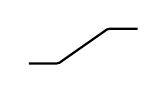
\begin{tikzpicture}[scale=0.22]
                \draw [thick] plot[domain=-pi:pi, samples=40] (\x, {min(1,max(-1, \x*0.7))});
            \end{tikzpicture}
        };

        % Summing junction
        \node [sum, right=1.0cm of sat] (sum1) {};
        \node at ($(sum1.west)+(0.18, 0.08)$)  {\tiny $+$};
        \node at ($(sum1.south)+(0.10, 0.18)$) {\tiny $-$};

        % Gain block
        \node [gainR, right=0.8cm of sum1, label=below:{\small Gain}] (gain) {$\frac{1}{5}$};

        % Integrator block
        \node [block, right=1.0cm of gain, label=below:{\small Integrator}] (int1) {$\dfrac{1}{s}$};

        % To Workspace
        \node [outblock, right=1.2cm of int1, label=below:{\small To Workspace}] (ws) {\small simout};

        % Trigonometric Function block (feedback, below)
        \node [block, below=1.4cm of gain, label=below:{\small Trigonometric\newline Function}] (trig) {\small sin};

        % Tap between int1 and ws
        \coordinate (tap) at ($(int1.east)!0.5!(ws.west)$);
        \filldraw (tap) circle (1.5pt);

        % Forward connections
        \draw [->] (sine)  -- (sat);
        \draw [->] (sat)   -- (sum1);
        \draw [->] (sum1)  -- (gain);
        \draw [->] (gain)  -- (int1);
        \draw [->] (int1)  -- (ws);

        % Feedback: tap -> trig -> sum1.south
        \draw [->] (tap) |- (trig.east);
        \draw [->] (trig.west) -| (sum1.south);

    \end{tikzpicture}
    }
    \caption{Simulink Block Diagram}
\end{figure}

%-----------------------------------
\myproblem{Problem 25}
Use Transfer Function blocks to plot solutions for $0 \le t \le 2$:
\[3\ddot{x} + 15\dot{x} + 18x = f(t),\quad x(0)=\dot{x}(0)=0\]
\[2\ddot{y} + 16\dot{y} + 50y = x(t),\quad y(0)=\dot{y}(0)=0\]
where $f(t) = 75\,u_s(t)$.

\textbf{Problem 25}

Use Transfer Function blocks to plot solutions for $0 \leq t \leq 2$:
\begin{align*}
    3\ddot{x} + 15\dot{x} + 18x &= f(t), \quad x(0) = \dot{x}(0) = 0 \\
    2\ddot{y} + 16\dot{y} + 50y &= x(t), \quad y(0) = \dot{y}(0) = 0
\end{align*}
where $f(t) = 75\,u_s(t)$.

\textbf{Solution:} Taking the Laplace transform with zero initial conditions:
\begin{align*}
    X(s) &= \frac{1}{3s^2+15s+18} \cdot F(s) \\
    Y(s) &= \frac{1}{2s^2+16s+50} \cdot X(s)
\end{align*}
The input $f(t) = 75\,u_s(t)$ is a unit step scaled by 75. Connect a Step block
(amplitude $= 75$) into Transfer Fcn1, whose output feeds Transfer Fcn. Both $x(t)$
and $y(t)$ are collected via a Mux into the \texttt{simout} To~Workspace block.

\begin{figure}[H]
    \centering
    \resizebox{\textwidth}{!}{%
    \begin{tikzpicture}[>=Stealth, node distance=1cm and 1.4cm]
        \tikzset{
            stepblock/.style = {draw, rectangle, minimum height=1.1cm, minimum width=1.1cm, align=center},
            tfblock/.style   = {draw, rectangle, minimum height=1.2cm, minimum width=2.6cm, align=center},
            muxblock/.style  = {draw, rectangle, minimum height=1.4cm, minimum width=0.3cm,
                                align=center, fill=black},
            outblock/.style  = {draw, rectangle, minimum height=1.0cm, minimum width=1.4cm, align=center},
        }

        % Step block (amplitude = 75)
        \node [stepblock, label=below:{\small Step}] (step) {%
            \begin{tikzpicture}[scale=0.25]
                \draw [thick] (-1,-1) -- (-1,0) -- (0,0) -- (0,1) -- (1,1);
                \draw [dashed, thin] (-1,0) -- (1,0);
            \end{tikzpicture}
        };
        \node [below=0.05cm of step, yshift=0.4cm] {\tiny amp $= 75$};

        % Transfer Fcn 1
        \node [tfblock, right=1.2cm of step, label=below:{\small Transfer Fcn1}] (tf1) {%
            $\dfrac{1}{3s^2+15s+18}$
        };

        % Transfer Fcn 2
        \node [tfblock, right=1.4cm of tf1, label=below:{\small Transfer Fcn}] (tf2) {%
            $\dfrac{1}{2s^2+16s+50}$
        };

        % Mux block (solid black bar)
        \node [muxblock, right=1.4cm of tf2] (mux) {};

        % To Workspace
        \node [outblock, right=0.8cm of mux, label=below:{\small To Workspace}] (ws) {\small simout};

        % Tap coordinates
        \coordinate (tapX) at ($(tf1.east)!0.5!(tf2.west)$);
        \coordinate (tapY) at ($(tf2.east)!0.5!(mux.west)$);
        \filldraw (tapX) circle (1.5pt);
        \filldraw (tapY) circle (1.5pt);

        % Forward connections
        \draw [->] (step) -- (tf1);
        \draw [->] (tf1)  -- (tf2);
        \draw [->] (tf2.east) -- (mux.west);
        \draw [->] (mux)  -- (ws);

        % x(t) tap -> mux bottom input
        \draw [->] (tapX) -- ++(0,-1.6) -| (mux.south);

        % Wire labels
        \node [above, font=\small] at (tapX) {$x(t)$};
        \node [above, font=\small] at (tapY) {$y(t)$};

    \end{tikzpicture}
    }
    \caption{Simulink model for Problem 25}
\end{figure}

%-----------------------------------
\myproblem{Problem 28}
Create a Simulink model to plot the solution for $0 \le t \le 1$:
\[\frac{Y(s)}{F(s)} = \frac{4}{s+5}, \qquad f(t) = u_s(t) - u_s(t-1)\]

\begin{figure}[H]
    \centering
    \begin{tikzpicture}[>=Stealth, node distance=1cm and 1.2cm]
        \tikzset{
            stepblock/.style = {draw, rectangle, minimum height=1.1cm, minimum width=1.1cm, align=center},
            tfblock/.style   = {draw, rectangle, minimum height=1.1cm, minimum width=1.8cm, align=center},
            scope/.style     = {draw, rectangle, minimum height=1.1cm, minimum width=1.1cm, align=center},
            sum/.style       = {draw, circle, minimum size=0.8cm, inner sep=0pt},
        }

        % Step blocks with internal step-function shape
        \node [stepblock, label=above left:{\small set start\newline time to 0}] (step1) {%
            \begin{tikzpicture}[scale=0.25]
                \draw [thick] (-1,-1) -- (-1, 0) -- (0, 0) -- (0, 1) -- (1, 1);
                \draw [dashed, thin] (-1, 0) -- (1, 0);
            \end{tikzpicture}
        };

        \node [stepblock, below=1.4cm of step1,
               label=below left:{\small set start\newline time to 1}] (step2) {%
            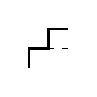
\begin{tikzpicture}[scale=0.25]
                \draw [thick] (-1,-1) -- (-1, 0) -- (0, 0) -- (0, 1) -- (1, 1);
                \draw [dashed, thin] (-1, 0) -- (1, 0);
            \end{tikzpicture}
        };

        % Summing junction (vertically centered between the two step blocks)
        \node [sum, right=1.2cm of step1, yshift=-0.8cm] (sum1) {};
        \node at ($(sum1.west)+(0.18, 0.08)$)  {\tiny $+$};
        \node at ($(sum1.south)+(0.10, 0.18)$) {\tiny $+$};

        % Transfer function block
        \node [tfblock, right=1.0cm of sum1] (tf) {$\dfrac{4}{s+5}$};

        % Scope
        \node [scope, right=1.2cm of tf] (scope) {$\square$};

        % Connections
        \draw [->] (step1.east) -- ++(0.4,0) |- (sum1.west);
        \draw [->] (step2.east) -- ++(0.4,0) |- (sum1.south);
        \draw [->] (sum1) -- (tf);
        \draw [->] (tf)   -- (scope);

    \end{tikzpicture}
    \caption{Simulink Block Diagram}
\end{figure}


%-----------------------------------
\myproblem{Problem 33}
Create a Simulink model for a mass supported by a nonlinear hardening spring, $0 \le t \le 2$:
\[5\ddot{y} = 5g - (900y + 1700y^3), \qquad y(0)=0.5,\;\dot{y}(0)=0\]
Use $g = 9.81$ m/s$^2$.



%-----------------------------------
\myproblem{Problem 35}
The equation for water height $h$ in a spherical tank (radius $r = 3$ m) with drain (radius 2 cm, $C_d = 0.5$), $h(0) = 5$ m:
\[\pi(2rh - h^2)\frac{dh}{dt} = -C_d A\sqrt{2gh}\]
Use Simulink to solve the nonlinear equation and plot $h(t)$ until $h(t) = 0$.

\begin{figure}[H]
    \centering
    \begin{tikzpicture}[>=Stealth, node distance=1cm and 1.2cm]
        \tikzset{
            block/.style   = {draw, rectangle, minimum height=1.0cm, minimum width=1.0cm, align=center},
            outblock/.style= {draw, rectangle, minimum height=0.9cm, minimum width=1.4cm, align=center},
        }

        % Integrator block
        \node [block, label=below:{\small Integrator}] (int1) {$\dfrac{1}{s}$};

        % To Workspace block
        \node [outblock, right=1.2cm of int1, label=below:{\small To Workspace}] (ws) {\small simout};

        % Fcn block (feedback, below)
        \node [block, below=1.2cm of int1, label=below:{\small Fcn}] (fcn) {$f(u)$};

        % Tap coordinate between int1 and ws
        \coordinate (tap) at ($(int1.east)!0.5!(ws.west)$);
        \filldraw (tap) circle (1.5pt);

        % Forward connections
        \draw [->] (int1) -- (ws);

        % Input arrow into integrator
        \draw [->] ($(int1.west)+(-0.8,0)$) -- (int1.west);

        % Feedback: tap -> down -> fcn
        \draw [->] (tap) |- (fcn.east);

        % Fcn output -> back to integrator input
        \draw [->] (fcn.west) -- ++(-0.8,0) |- (int1.west);

    \end{tikzpicture}
    \caption{Simulink Block Diagram}
\end{figure}

%-----------------------------------
\myproblem{Problem 45}
Consider the system in Figure P45 with $m_1=m_2=1$, $c_1=3$, $c_2=1$, $k_1=1$, $k_2=4$:
\[m_1\ddot{x}_1 + (c_1+c_2)\dot{x}_1 + (k_1+k_2)x_1 - c_2\dot{x}_2 - k_2x_2 = 0\]
\[m_2\ddot{x}_2 + c_2\dot{x}_2 + k_2x_2 - c_2\dot{x}_1 - k_2x_1 = f(t)\]
\begin{itemize}
    \item[a.] Develop a Simulink model using state-variable representation.
    \item[b.] Plot $x_1(t)$ for zero initial conditions with piecewise input:
    \[f(t) = \begin{cases} t & 0 \le t \le 1 \\ 2-t & 1 < t < 2 \\ 0 & t \ge 2 \end{cases}\]
\end{itemize}


\begin{figure}[H]
    \centering
    \begin{tikzpicture}[>=Stealth, node distance=1cm and 1.2cm]
        \tikzset{
            rampblock/.style = {draw, rectangle, minimum height=1.1cm, minimum width=1.1cm, align=center},
            ssblock/.style   = {draw, rectangle, minimum height=1.4cm, minimum width=2.0cm, align=center},
            outblock/.style  = {draw, rectangle, minimum height=1.0cm, minimum width=1.4cm, align=center},
            sum/.style       = {draw, circle, minimum size=0.8cm, inner sep=0pt},
        }

        % Ramp blocks with diagonal line inside
        \node [rampblock, label=below:{\small Ramp}]  (ramp0) {%
            \begin{tikzpicture}[scale=0.25]
                \draw [thick] (-1,-1) -- (1,1);
            \end{tikzpicture}
        };
        \node [rampblock, below=0.8cm of ramp0, label=below:{\small Ramp1}] (ramp1) {%
            
\begin{tikzpicture}[scale=0.25]
                \draw [thick] (-1,-1) -- (1,1);
            \end{tikzpicture}
        };
        \node [rampblock, below=0.8cm of ramp1, label=below:{\small Ramp2}] (ramp2) {%
            
\begin{tikzpicture}[scale=0.25]
                \draw [thick] (-1,-1) -- (1,1);
            \end{tikzpicture}
        };

        % Summing junction aligned with ramp1
        \node [sum, right=1.2cm of ramp1] (sum1) {};
        \node at ($(sum1.north)+(0.10,-0.18)$) {\tiny $+$};
        \node at ($(sum1.west)+(0.18, 0.08)$)  {\tiny $+$};
        \node at ($(sum1.south)+(0.10, 0.18)$) {\tiny $+$};

        % State-Space block
        \node [ssblock, right=1.2cm of sum1, label=below:{\small State-Space}] (ss) {%
            \small $x' = Ax+Bu$\\
            \small $y = Cx+Du$
        };

        % To Workspace
        \node [outblock, right=1.2cm of ss, label=below:{\small To Workspace}] (ws) {\small simout};

        % Connections
        \draw [->] (ramp0.east) -- ++(0.4,0) |- (sum1.north);
        \draw [->] (ramp1.east) -- (sum1.west);
        \draw [->] (ramp2.east) -- ++(0.4,0) |- (sum1.south);
        \draw [->] (sum1) -- (ss);
        \draw [->] (ss)   -- (ws);

    \end{tikzpicture}
    \caption{Simulink Block Diagram}
\end{figure}